\begin{figure*}[ht]
    \centering
    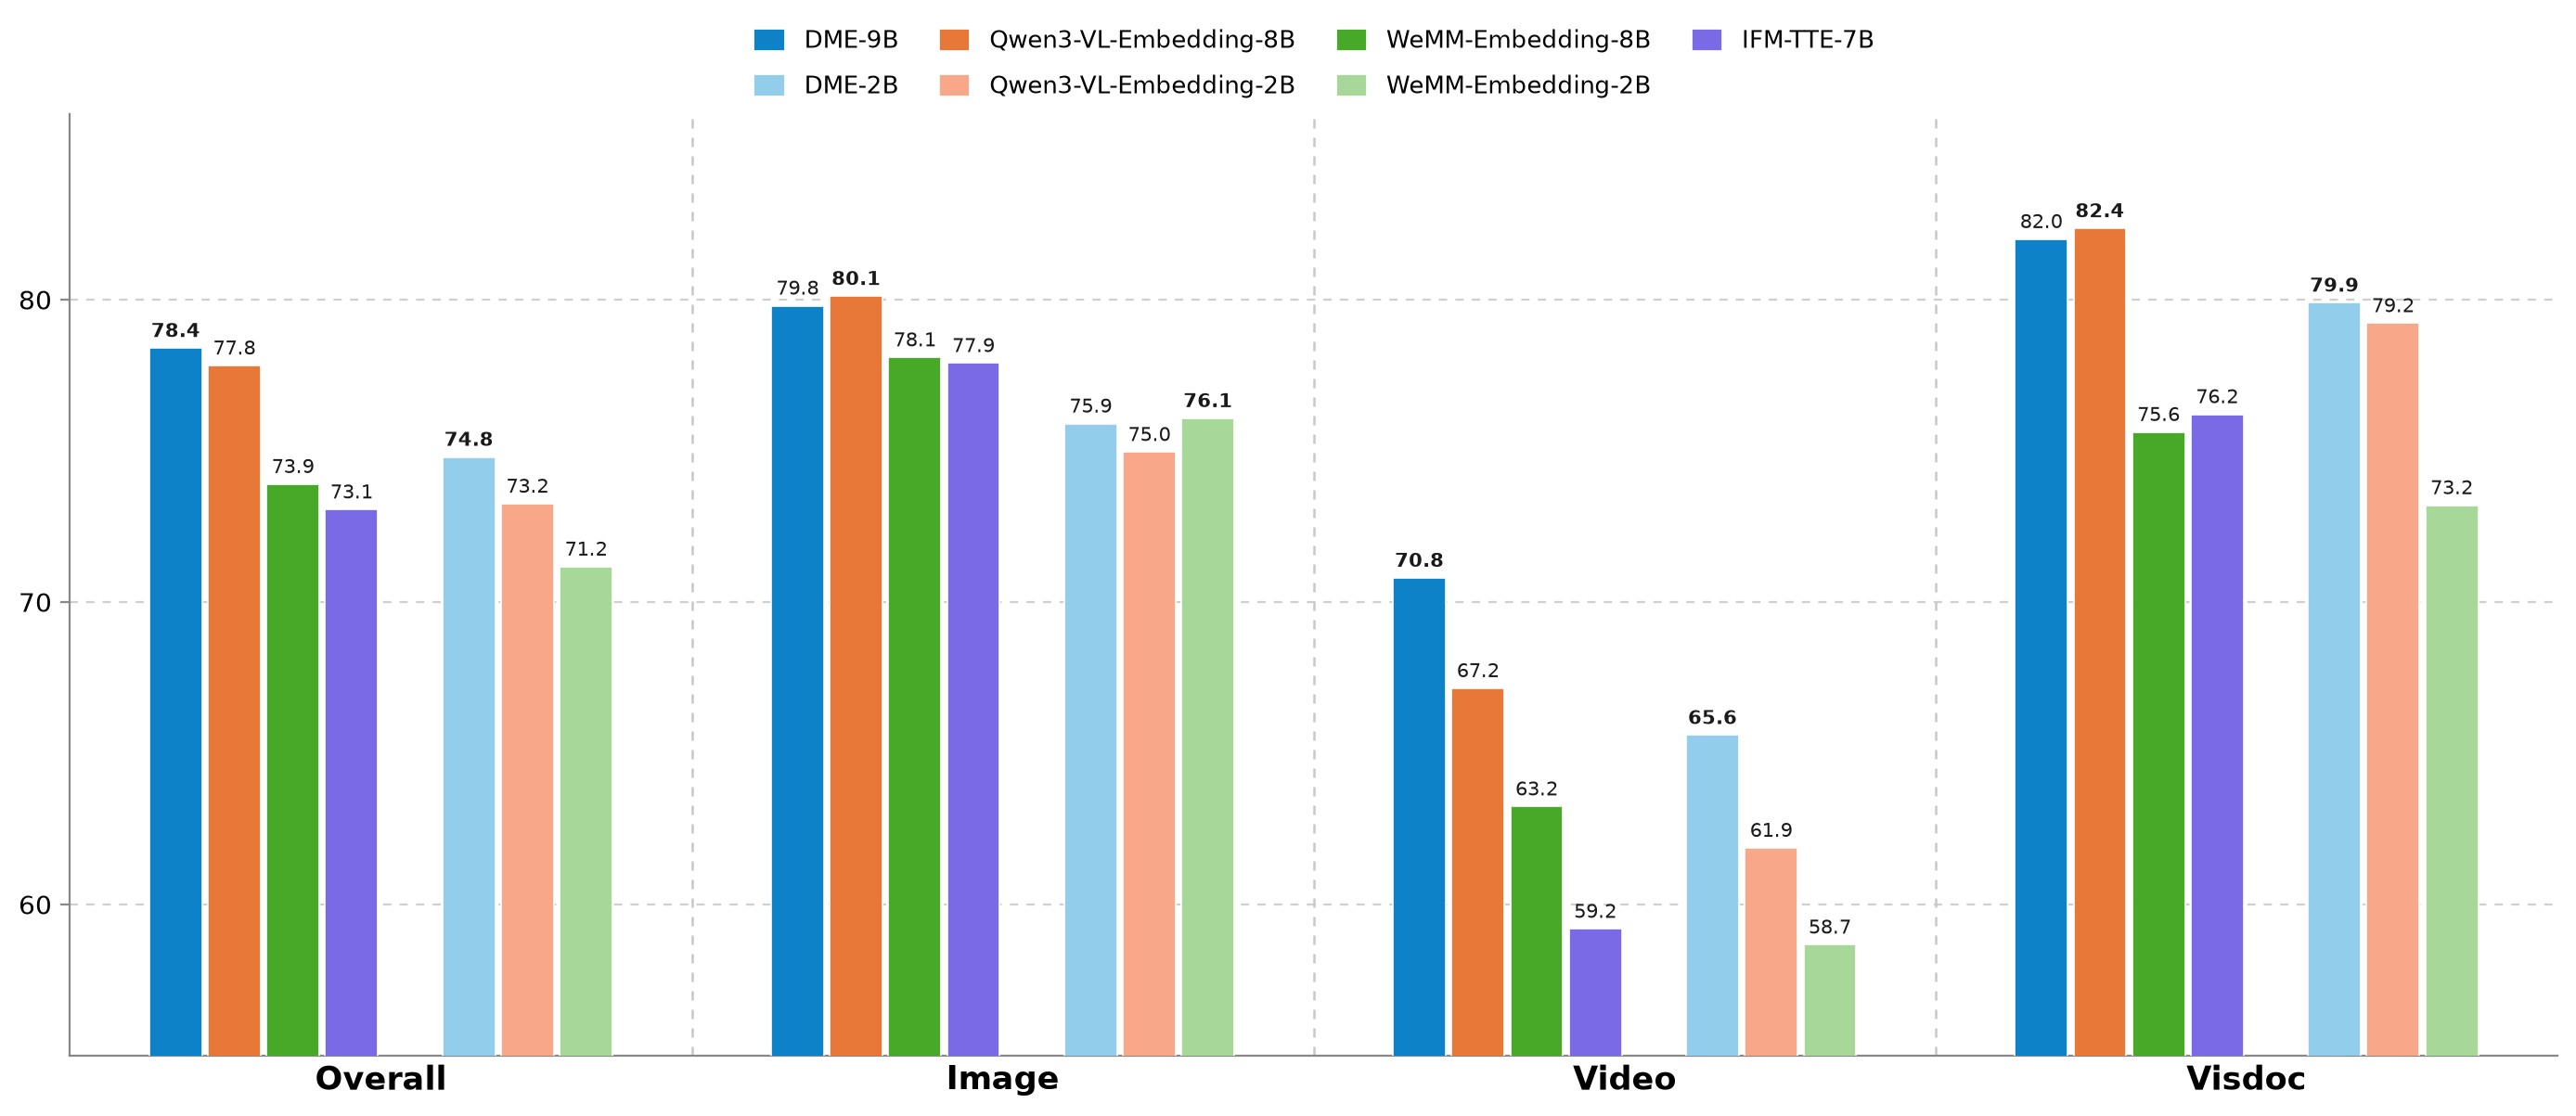
\includegraphics[width=1\linewidth]{figures/fig-performance.png}
    \caption{\textbf{Performance Comparison.} Overall and per-domain (Image, Video, VisDoc) results on MMEB-v2. At both the 2B and 9B scales, DME consistently outperforms other embedding models with especially large gains on video and visual-document retrieval.}
  \label{fig:performance}
\end{figure*}

\section{Introduction}
\label{sec:introduction}

Multimodal retrieval has become a central infrastructure for modern search and recommendation systems, and increasingly powers the retrieval tools of modern agents. In these systems, both user intents and candidate contents may appear as text, images, videos, visual documents, or their arbitrary mixtures. This requirement is further amplified on large-scale video and image--text platforms such as Douyin, Xiaohongshu, and YouTube, where real-world content is massive in scale and highly heterogeneous. User queries may be expressed through natural language, images, videos, or mixed-modality inputs, while candidate items may contain visual frames, video dynamics, OCR text, captions, metadata, and other textual signals. A practical retrieval model must therefore satisfy two requirements simultaneously: it should provide broad modality and task coverage under massive-scale indexing, while still preserving fine-grained semantic discrimination for difficult query--document matching.

Early vision-language contrastive models such as CLIP and ALIGN demonstrate that large-scale paired supervision can induce strong cross-modal alignment~\cite{CLIP,ALIGN}. More recently, frontier MLLMs such as Qwen3-VL and Qwen3.5 have become increasingly attractive as foundation backbones for multimodal embedding, as they provide stronger visual-language understanding, instruction following, long-context modeling, and multimodal reasoning ability~\cite{Qwen3VL,Qwen35Blog}. Building on these foundation models, recent MLLM-based embedding systems adapt generative MLLMs into unified multimodal retrievers over text, images, videos, visual documents, and mixed-modality inputs~\cite{E5-V,GME,mme5,u-marvel,VLM2VecV2,Qwen3VLEmbedding}, and have become the mainstream paradigm for universal multimodal retrieval.

The dominant recipe for training these MLLM-based retrievers is still contrastive learning. Positive query--document pairs are pulled together, while negatives are pushed apart in the embedding space~\cite{infonce,CLIP,E5,GTE}. This paradigm is scalable, compatible with offline corpus encoding, and well aligned with industrial vector-search systems. However, we argue that contrastive MLLM embedders face an inherent tension: they inherit the strong perception and reasoning potential of generative MLLMs, but use the model mainly as an encoder optimized by pair-level similarity supervision. Such supervision tells the model which instances should be close, but does not explicitly specify why they are relevant, which local evidence supports the relevance decision, or what fine-grained counterpart information should be preserved in the final embedding.

This limitation becomes more critical in large-scale industrial multimodal retrieval. Many real queries are not simple category or caption matching requests; they may involve multiple constraints over objects, attributes, actions, OCR text, temporal order, or spatial relations. At the same time, hard negatives often share the same global scene or topic with the positive document, and differ only in a small visual region, a key frame, a local text span, or a subtle semantic condition~\cite{unime}. Recent benchmarks have therefore moved beyond conventional image--text retrieval toward video, visual-document, moment, and reasoning-intensive retrieval~\cite{VLM2VecV2,ColPali,visrag,MMBright}, where such fine-grained, locally-grounded matching is especially demanding. In these scenarios, an embedding should not merely encode global similarity; it should be formed from retrieval-relevant evidence and preserve enough semantic detail to distinguish partially matched candidates.

Recent studies have explored how to reintroduce reasoning into multimodal retrieval representations. Some methods generate embedding-centric reasoning traces or let the model adaptively decide whether to emit a reasoning chain before the embedding token~\cite{ThinkThenEmbed,TRACE}, while others use retrieval-oriented reinforcement learning to drive reasoning-augmented generative embeddings~\cite{UMER1,EmbedRL}. These methods show that reasoning can improve fine-grained retrieval, but many rely on explicit textual reasoning
or reranking-style computation. Such designs are powerful but sacrifice efficiency, making them difficult to deploy as the main retrieval encoder in billion-scale online systems.

\begin{figure*}[tp]
    \centering
    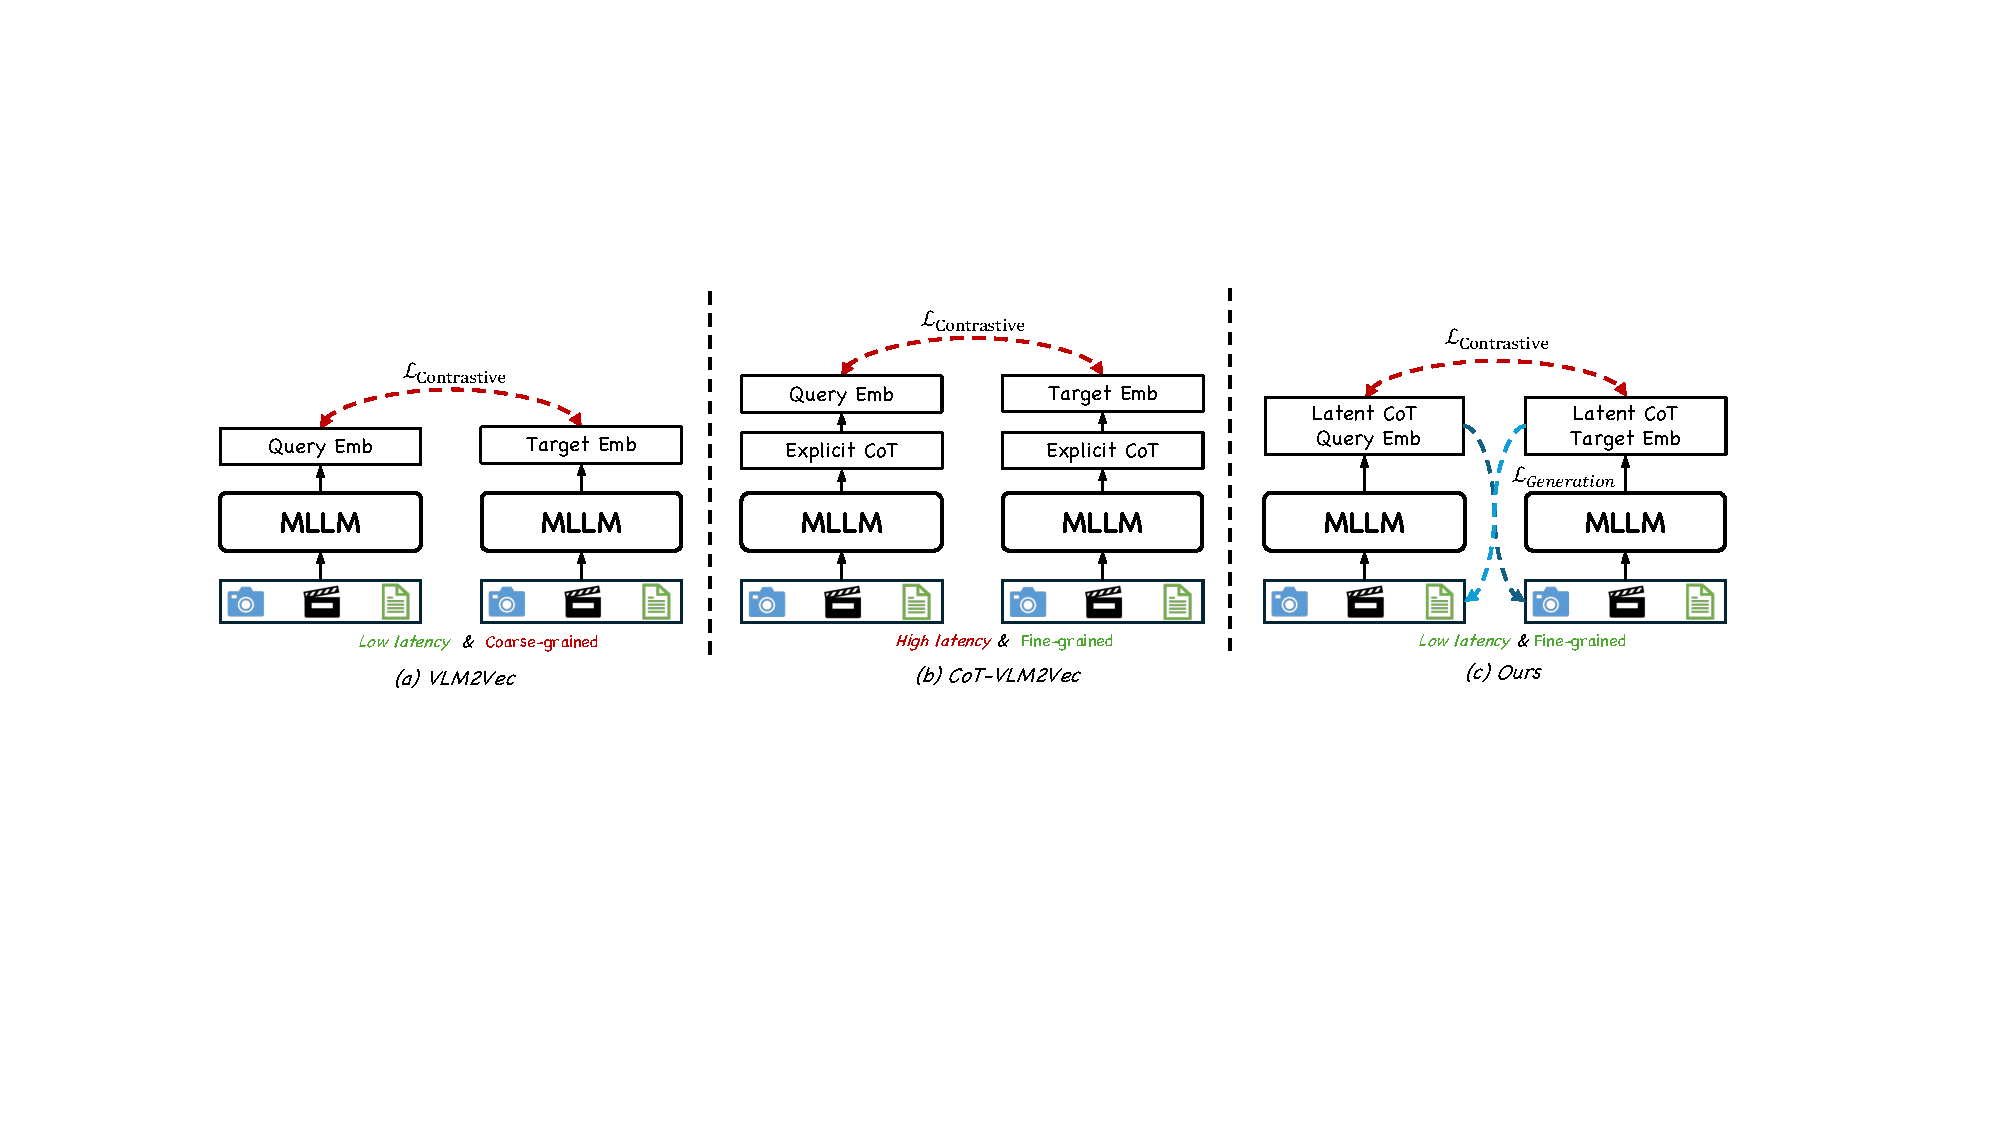
\includegraphics[width=1\linewidth]{figures/fig-compare.pdf}
\caption{\textbf{Comparison with prior works.} (a) Contrastive MLLM embedders (e.g., VLM2Vec) encode each side in a single pass, yielding \emph{low latency} but only \emph{coarse-grained} representations. (b) CoT-based embedders prepend explicit reasoning before the embedding, improving \emph{fine-grained} discrimination at the cost of \emph{high latency}. (c) DME performs latent reasoning together with cross-conditional generative supervision, achieving \emph{fine-grained} representations while retaining the \emph{low latency} of a bi-encoder.}
  \label{fig:comparison}
\end{figure*}



This creates two practical design requirements for industrial multimodal retrieval. First, the model should acquire evidence-aware reasoning ability without turning online retrieval into an explicit generation or reranking process, so that adding reasoning capacity introduces only marginal query-encoding overhead. 
Second, the representation itself must retain enough fine-grained counterpart-side detail to separate hard negatives, since even the right evidence can collapse into a single vector that drops such detail. Crucially, both abilities should be obtained without explicit generation or additional model passes, so that retrieval preserves the standard dense-vector interface.

Motivated by this industrial gap, we introduce Douyin Multimodal Embedding (DME), a two-stage multimodal embedding model designed to meet the two requirements above by combining the efficiency of contrastive MLLM embedders with the fine-grained semantic modeling ability of reasoning-augmented retrievers. Stage 1 performs large-scale contrastive pre-training over heterogeneous multimodal data, establishing a broad unified embedding space across text, images, videos, visual documents, and mixed-modality inputs. Stage 2 then improves the semantic sufficiency of the learned embeddings. We use semantic sufficiency to describe a stronger requirement for retrieval representations: an embedding should be not only pairwise aligned with relevant instances, but also grounded in retrieval-relevant evidence and capable of preserving fine-grained counterpart semantics from the matched query or document.

To achieve this goal, Stage 2 introduces two complementary mechanisms. The first is Evidence-Grounded Typed Latent Reasoning, which injects a controllable hidden-space reasoning process into the embedding model. Instead of generating explicit long-form CoT, DME uses latent tokens to organize retrieval computation before the final embedding readout. Anchor tokens first localize retrieval-relevant evidence from multimodal inputs, such as text spans, image regions, OCR fragments, or video keyframes. Typed latent reasoning states then organize the localized evidence into
retrieval-specific roles, including semantic localization, positive alignment,
and negative rejection. Teacher-generated trajectories may additionally contain
summarization states. Finally, a readout representation fuses the latent reasoning states and evidence representations into the final retrieval embedding. This design introduces the structure of evidence localization, latent reasoning, and embedding readout into multimodal retrieval, while preserving the efficiency of a bi-encoder model.

The second Stage-2 mechanism is Cross-Conditional Reconstruction, which combines Next Token Prediction (NTP) and Multi-Token Prediction (MTP). Reconstruction and generative supervision have long been used to improve representations, from masked language and image modeling to contrastive-captioning objectives~\cite{bert,MAE,CoCa}. Recent multimodal embedding studies further show that content reconstruction or joint generative-retrieval training can encourage MLLMs to compress richer semantic information into embedding tokens~\cite{CoCoA,CREM}. Inspired by this direction, DME uses the retrieval embedding itself as a semantic bottleneck for generation-oriented supervision. Given a positive query--document pair, the query embedding is used as a prefix condition to reconstruct document-side textual content, and the document embedding is symmetrically used to reconstruct query-side textual content. MTP further extends this signal by predicting multiple future tokens rather than only the next token, encouraging the embedding to capture longer-range semantic information~\cite{MultiTokenPrediction,DeepSeekV3}. These objectives provide fine-grained token-level supervision during training, without requiring additional decoding during retrieval inference. A further benefit of this generative supervision is that the token-level content of the input can be recovered from its embedding. We quantify this as a representation completeness measure, giving an interpretable measure of semantic sufficiency and an explicit signal to guide representation optimization.

Together, the two Stage-2 components address the two requirements above. Evidence-Grounded Typed Latent Reasoning improves how an embedding is formed: it encourages the model to look at the right evidence, organize retrieval-specific latent states, and fuse them into the final vector. Cross-Conditional Reconstruction improves what an embedding must preserve: it requires the vector representation to retain enough counterpart-side semantics to support conditional textual reconstruction. Both mechanisms are used to improve the embedding model itself. At inference time, DME remains an efficient bi-encoder retriever: each query or document is independently encoded into a dense vector, and retrieval is performed by vector similarity without explicit reasoning generation, agentic tool use, or cross-encoder scoring.

The main contributions of this report are summarized as follows:
\begin{itemize}
    \item We present Douyin Multimodal Embedding (DME), a two-stage multimodal embedding model for large-scale industrial multimodal retrieval. DME combines large-scale contrastive pre-training with semantic sufficiency learning, aiming to preserve bi-encoder efficiency while improving fine-grained multimodal understanding.

    \item We introduce two complementary Stage-2 mechanisms for semantic sufficiency: Evidence-Grounded Typed Latent Reasoning, which grounds embeddings in localized evidence through anchor-based hidden-space reasoning, and Cross-Conditional Reconstruction, which uses NTP and MTP to inject counterpart-side semantic supervision, so that the input content can be recovered from its embedding.

    \item We train and evaluate DME at both 2B and 9B scales. On MMEB-v2, DME-2B and DME-9B achieve state-of-the-art results among models of comparable sizes, with especially strong performance on video and visual-document retrieval (Figure~\ref{fig:performance}), while the latent reasoning tokens introduce only minor query-encoding latency overhead. We further show, through a token-level recovery analysis that we formalize as a representation completeness measure, that DME embeddings are information-complete, giving direct evidence of semantic sufficiency. Deployed in Douyin's real-world retrieval system, DME delivers a 2.92\% relative improvement in overall score on the in-house offline evaluation set, with consistent gains across all cross-modal retrieval directions, and has been adopted across a range of scenarios such as generative search, image search, and AI search. Online A/B testing on Douyin search further confirms a 0.1\% Lifetime (LT) gain.
\end{itemize}

The report is organized as follows. Section~\ref{sec:dme-overview} provides an overview of the DME architecture, retrieval setting, embedding extraction, and two-stage learning pipeline. Section~\ref{sec:multi-stage-learning-framework} describes the multi-stage learning framework in detail, including large-scale contrastive pre-training and the two Stage-2 semantic sufficiency mechanisms. Section~\ref{sec:experiments} presents the experimental setup, main results, and analysis. Section~\ref{sec:conclusion} concludes the report and discusses future directions.